\documentclass{article}[12pt]
\usepackage{amsmath}
\usepackage{gensymb}
\usepackage{standalone}
\usepackage{verbatim}
\usepackage[utf8]{inputenc}
\usepackage{setspace}
\usepackage[a4paper,margin=1in,footskip=0.25in]{geometry}
\usepackage{graphicx}
\usepackage{mathptmx}
\usepackage{booktabs}
\usepackage{cite}
\usepackage[english]{babel}
\usepackage[utf8]{inputenc}

\begin{document}
\section{Code Validation}
	To verify the functionality and accuracy of the implemented code a simple two terminal device was used. The geometry was set to be a $100\mu m$ square with $100$ nodes on each axis. The terminals were placed across the top and bottom surfaces, with the top having an applied voltage of $1000V$ and the bottom being set to ground. Solving of Poisson's equation for this geometry results in a linear relationship. \\ \\
 	\noindent
 The simulated results of the two terminal device is seen in Figure \ref{fig:two_terminal}. As can be seen the simulated results show a linear relationship between voltage and distance in $y$.
 
 \begin{figure}[h!]
 	\centering
 	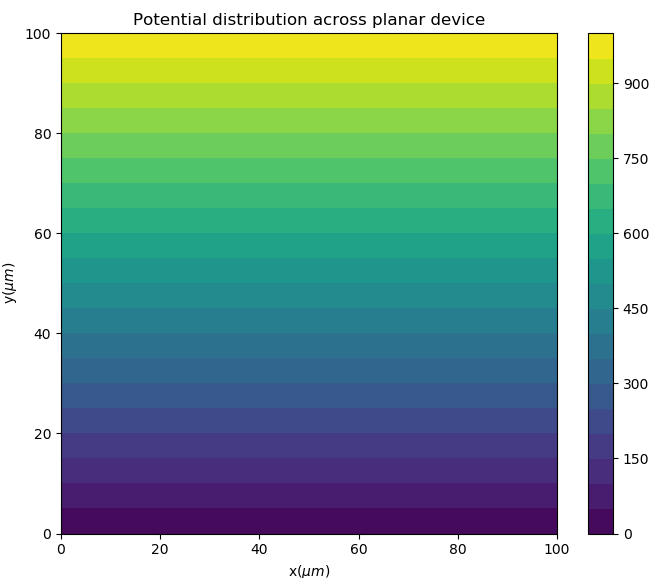
\includegraphics[width=\linewidth]{two_terminal1.png}
 	\caption{Simulated voltage distribution of two terminal device.}
 	\label{fig:two_terminal}
\end{figure}
\end{document}
